\chapter{Jet Results and Outlook} \label{ch:cando}

\section{8 TeV Inclusive Jet Results and Discussion}

\subsubsection{Differential Jet Cross-Section}

\afterpage{%

\begin{figure}
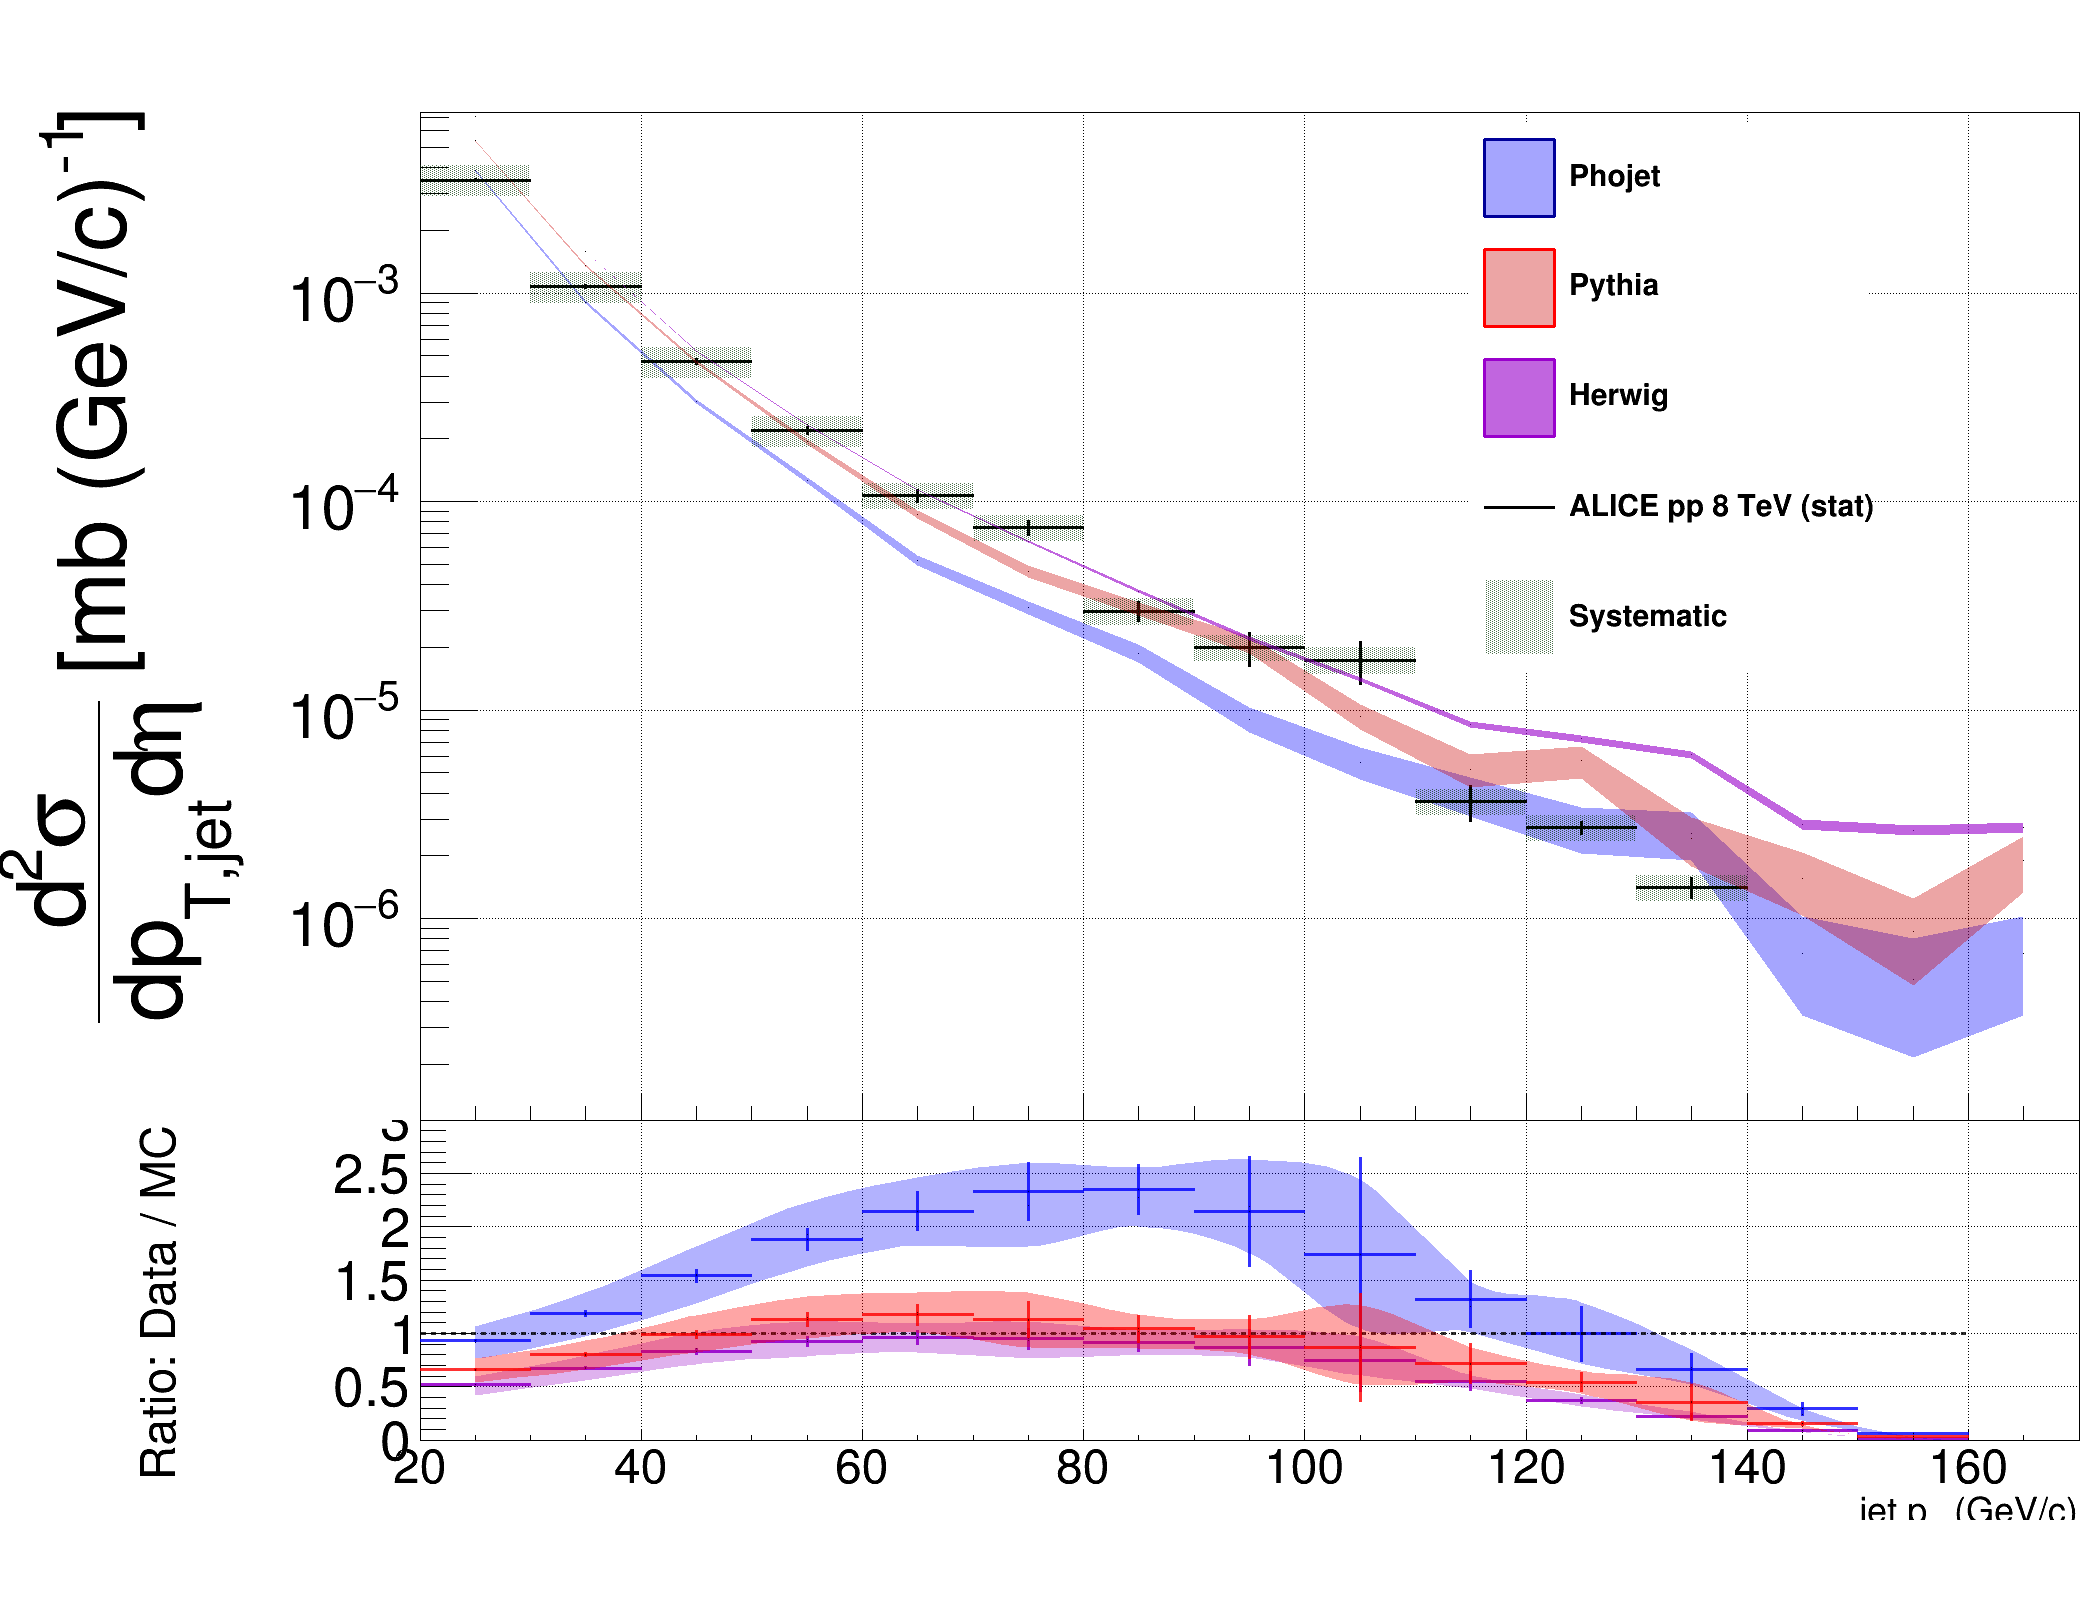
\includegraphics[width=\linewidth]{XSecR02}
\centering
\caption{8 TeV inclusive jet differential cross-section for R = 0.2.}
\label{fig:JetXsecR02}
\end{figure}

\begin{figure}
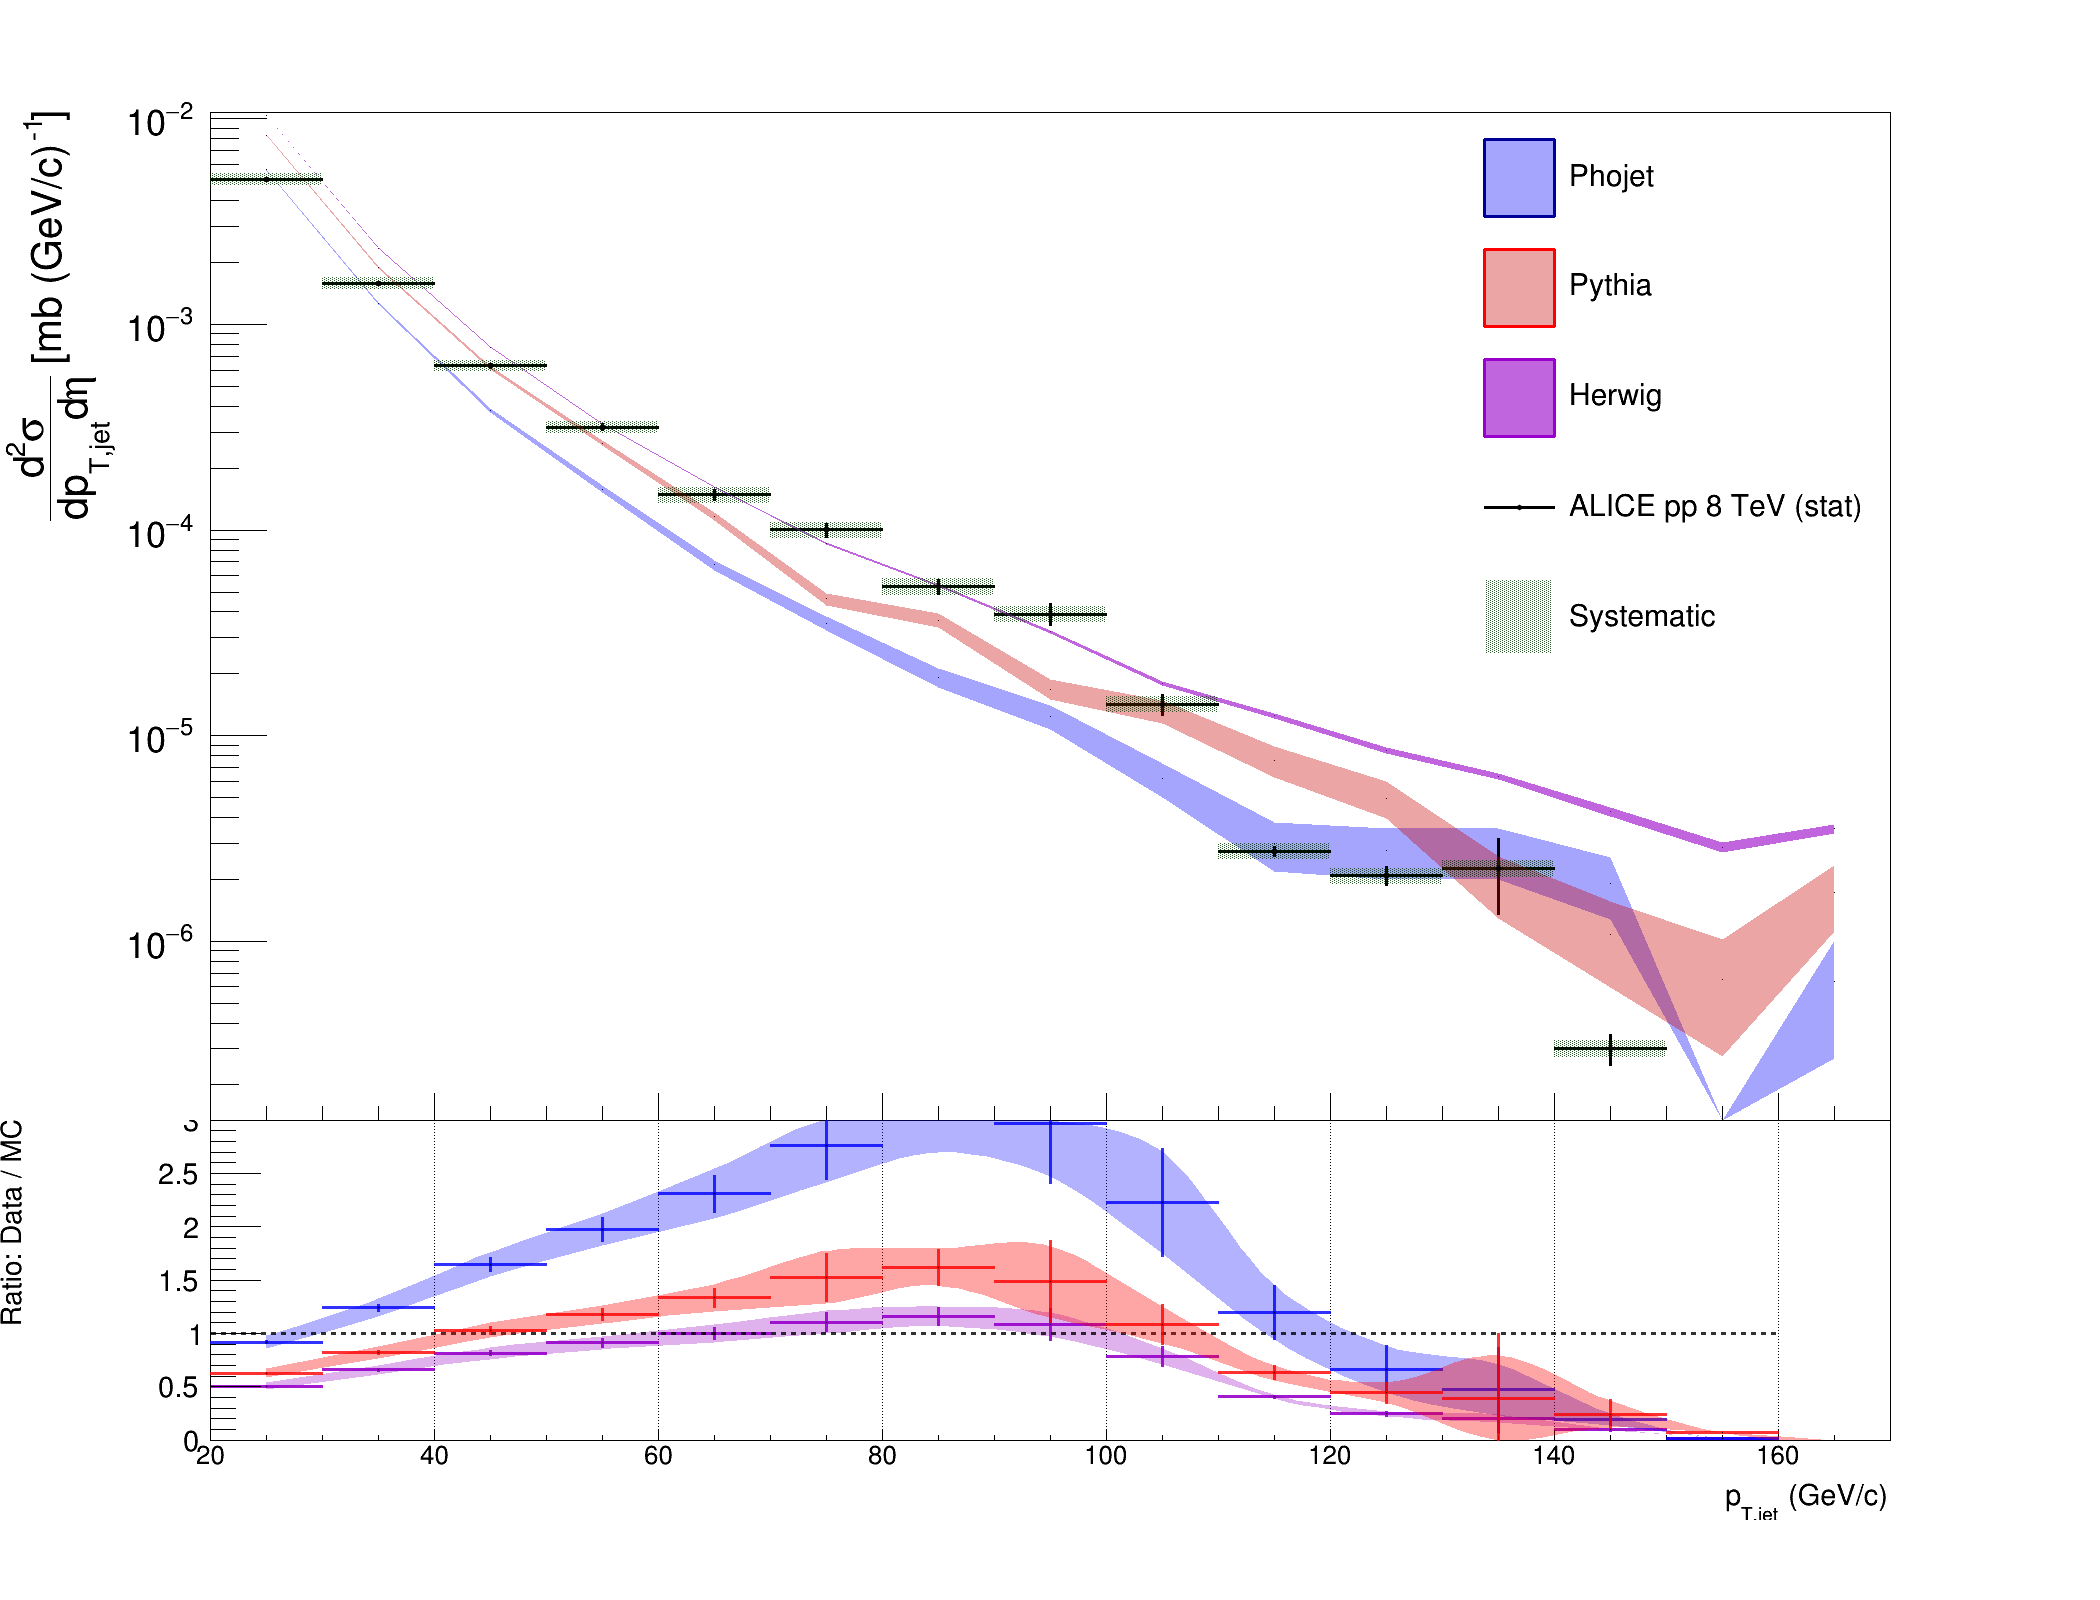
\includegraphics[width=\linewidth]{XSecR03}
\centering
\caption{8 TeV inclusive jet differential cross-section for R = 0.3.}
\label{fig:JetXsecR03}
\end{figure}

\begin{figure}
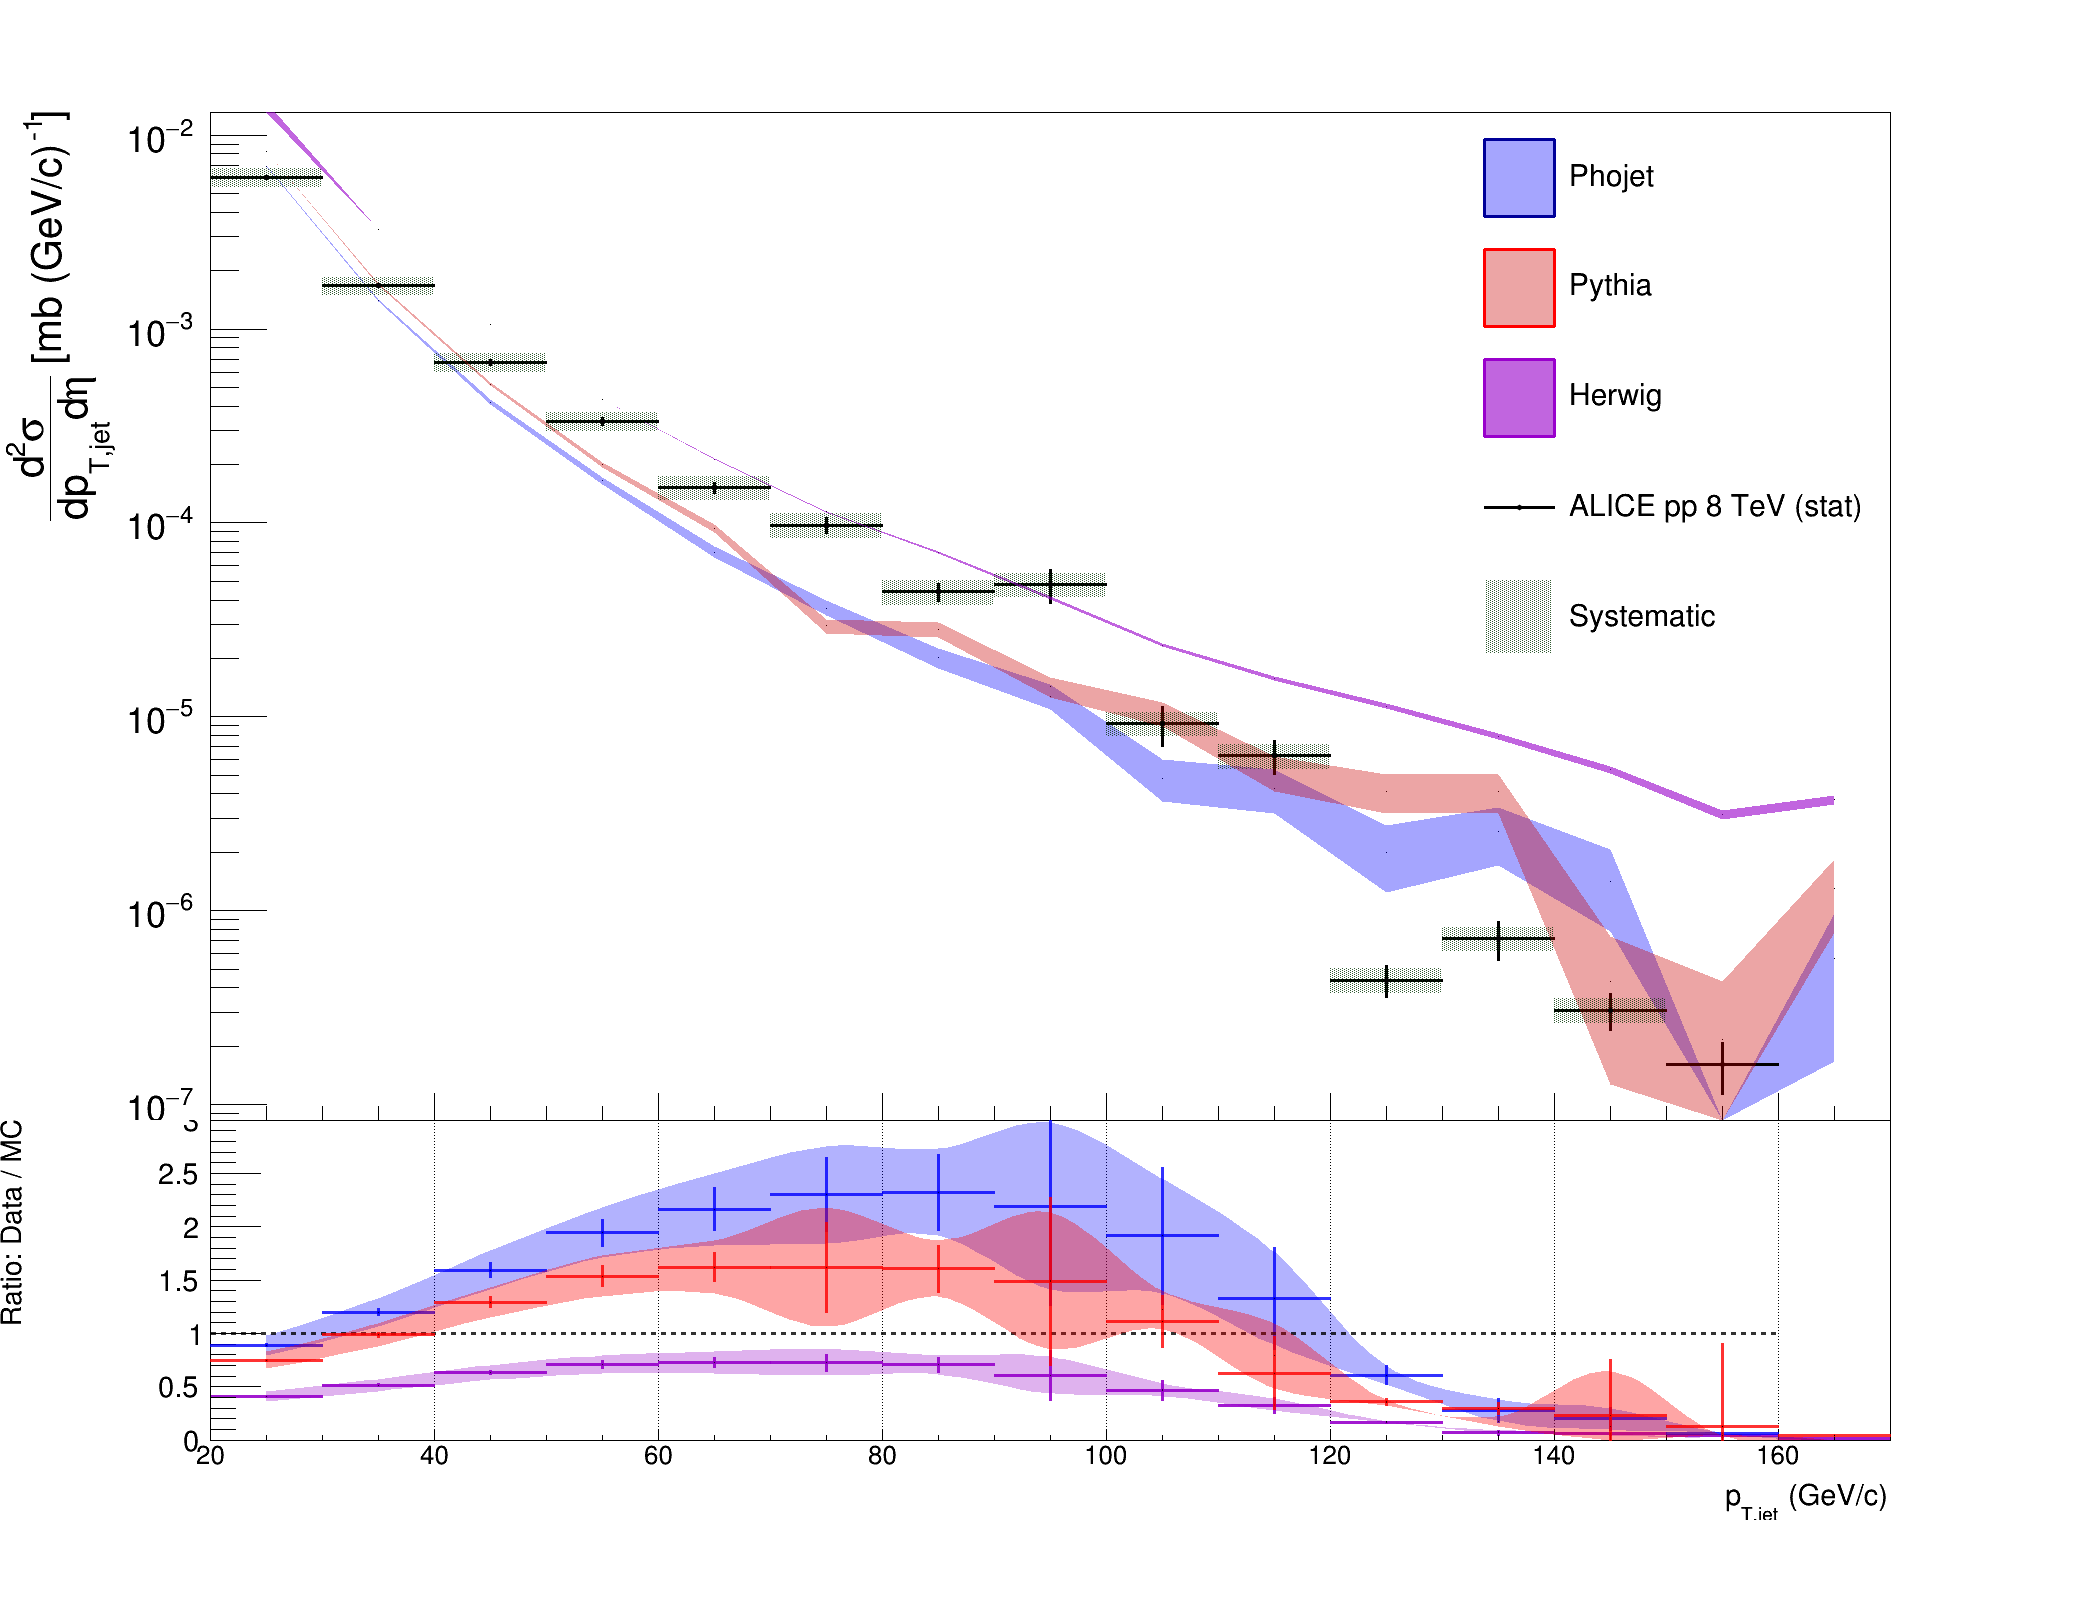
\includegraphics[width=\linewidth]{XSecR04}
\centering
\caption{8 TeV inclusive jet differential cross-section for R = 0.4.}
\label{fig:JetXsecR04}
\end{figure}

\clearpage
}

\noindent
Figures \ref{fig:JetXsecR02}, \ref{fig:JetXsecR03}, and \ref{fig:JetXsecR04} show the inclusive jet cross-sections from R = 0.2 through R = 0.4 jet radii.  The figures are split into two sections.  The cross-sections as measured from ALICE along with the associated statistical errors are shown in black.  The associated systematic errors from the ALICE data as discussed in this chapter are shown as the green shaded area.  Min Bias Monte Carlo generated events from Pythia (Red), PHOjet (blue), and Herwig (magenta) are included and shown as colored bands to convey the statistical uncertainties from each simulation.  On the bottom half of each plot are the relative ratios of the ALICE jet cross-sections to one of the Monte Carlos using the same color scheme as above.  

What can we tell from these results?  First, we can see that the cross-sections are measured over a wide range, about five orders of magnitude, between 20 GeV/\textit{c} to 160 GeV/\textit{c} in $p_{T}$.  The R = 0.2 and R = 0.3 cross-sections show a well defined trend between 20 GeV/\textit{c} - $\sim$100 GeV/c, after this point the data  has a hard drop after which the data points show wider fluctuations.  This same trend is seen in the R = 0.4 jet cross-section but the jerk happens earlier in $p_{T}$ around  80 GeV/\textit{c}.  The fluctuations are an artifact of the bin-by-bin corrections and the lack of EMCal trigger simulations as discussed in Chapter \ref{ch:analysis}.  

Comparing the data to the Monte Carlos we see that the two simulations produced by the ALICE Collaboration, Pythia and PHOjet, tend to under predict the data.  PHOjet has the least agreement with the data.  The poor agreement with PHOjet can be explained by the fact that PHOjet is an older Monte Carlo generator and better tuned to describing lower energy experiments from the past.  PHOjet may also be under estimating the data because it focuses on describing photon interactions.  The Monte Carlo Simulation from Herwig was produced on a local server farm at the University of Tennessee.  I used a Min Bias tune of Herwig and generated 150 million events and we see that reflected in the low statistical errors.  The Herwig simulation tends to slightly over predict the data.  Both Herwig and Pythia agree well with the data between 20 GeV/c to 100 GeV/c.  It is hard to say that one is `better' then the other because of the relatively large statistical errors from Pythia.  However, for the R = 0.4 jet cross-section we can see that the data seems to trend better towards the clusterization description of hadronization used in Herwig.

Through scaling these results may serve as a reference for heavy-ion collisions and help to better constrain our understanding of parton energy loss mechanisms in the QGP.  


\subsubsection{Jet Cross-Section Ratios}


\noindent
The ratio of the jet cross-sections as a function of the jet radii is defined as,

\begin{equation}
\mathscr{R} (p_{T}; \, R_{1},R_{2}) = \frac{d\sigma(R_{1}) /d\eta \, dp_{T} }{d\sigma (R_{2}) /d\eta \, dp_{T}},
\label{eq:jetxsecratio}
\end{equation}

\noindent
where $R_{1}$ and $R_{2}$ are the jet radii in question. This probes the transverse structure of jets and is sensitive to QCD hardonization\cite{SOYEZ201159}.  Figures \ref{fig:JetXsecRatioR02}, \ref{fig:JetXsecRatioR03}, and \ref{fig:JetXsecRatioR023} report the ratios of the jet cross-sections between R = 0.2 / R = 0.4, R = 0.3 / R= 0.4, and R = 0.2 / R = 0.3 respectively.  The figures also show the relative ratios plotted from the 8 TeV ALICE data, Pythia, PHOjet, and Herwig using the same color schema as the jet cross-sections.  Errors between the cross-sections of different radii are considered uncorrelated and added in quadrature to form the error bars reported in the figures.

\afterpage{%

\begin{figure}
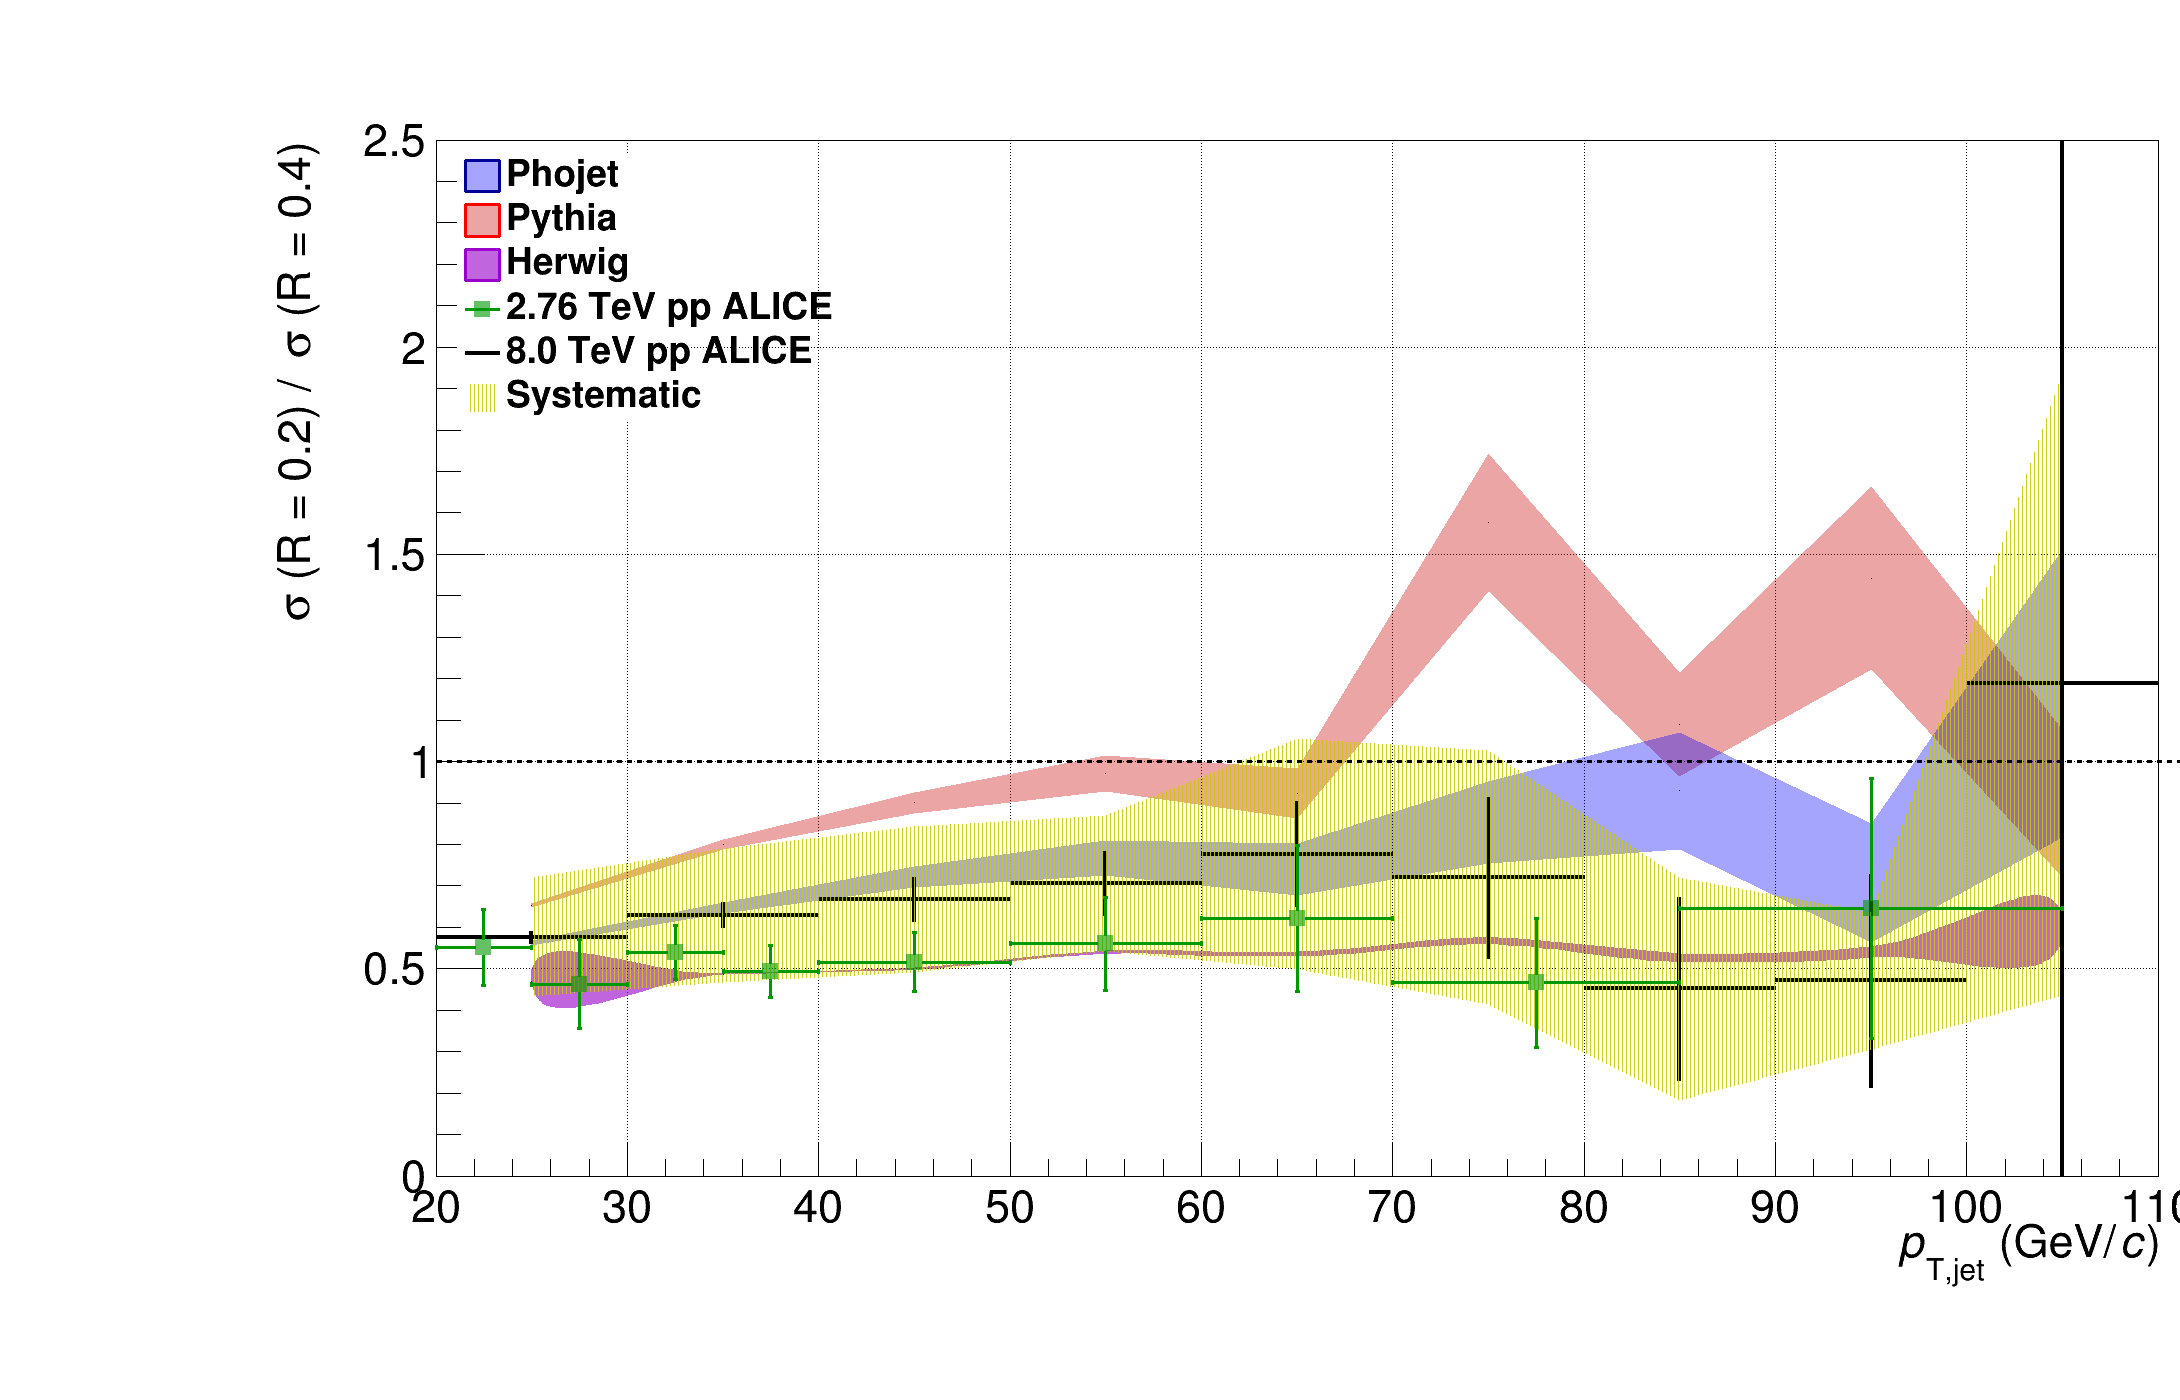
\includegraphics[width=\linewidth]{XSecRatioR02}
\centering
\caption{Ratio of the jet cross-sections R = 0.2  to R = 0.4.}
\label{fig:JetXsecRatioR02}
\end{figure}

\begin{figure}
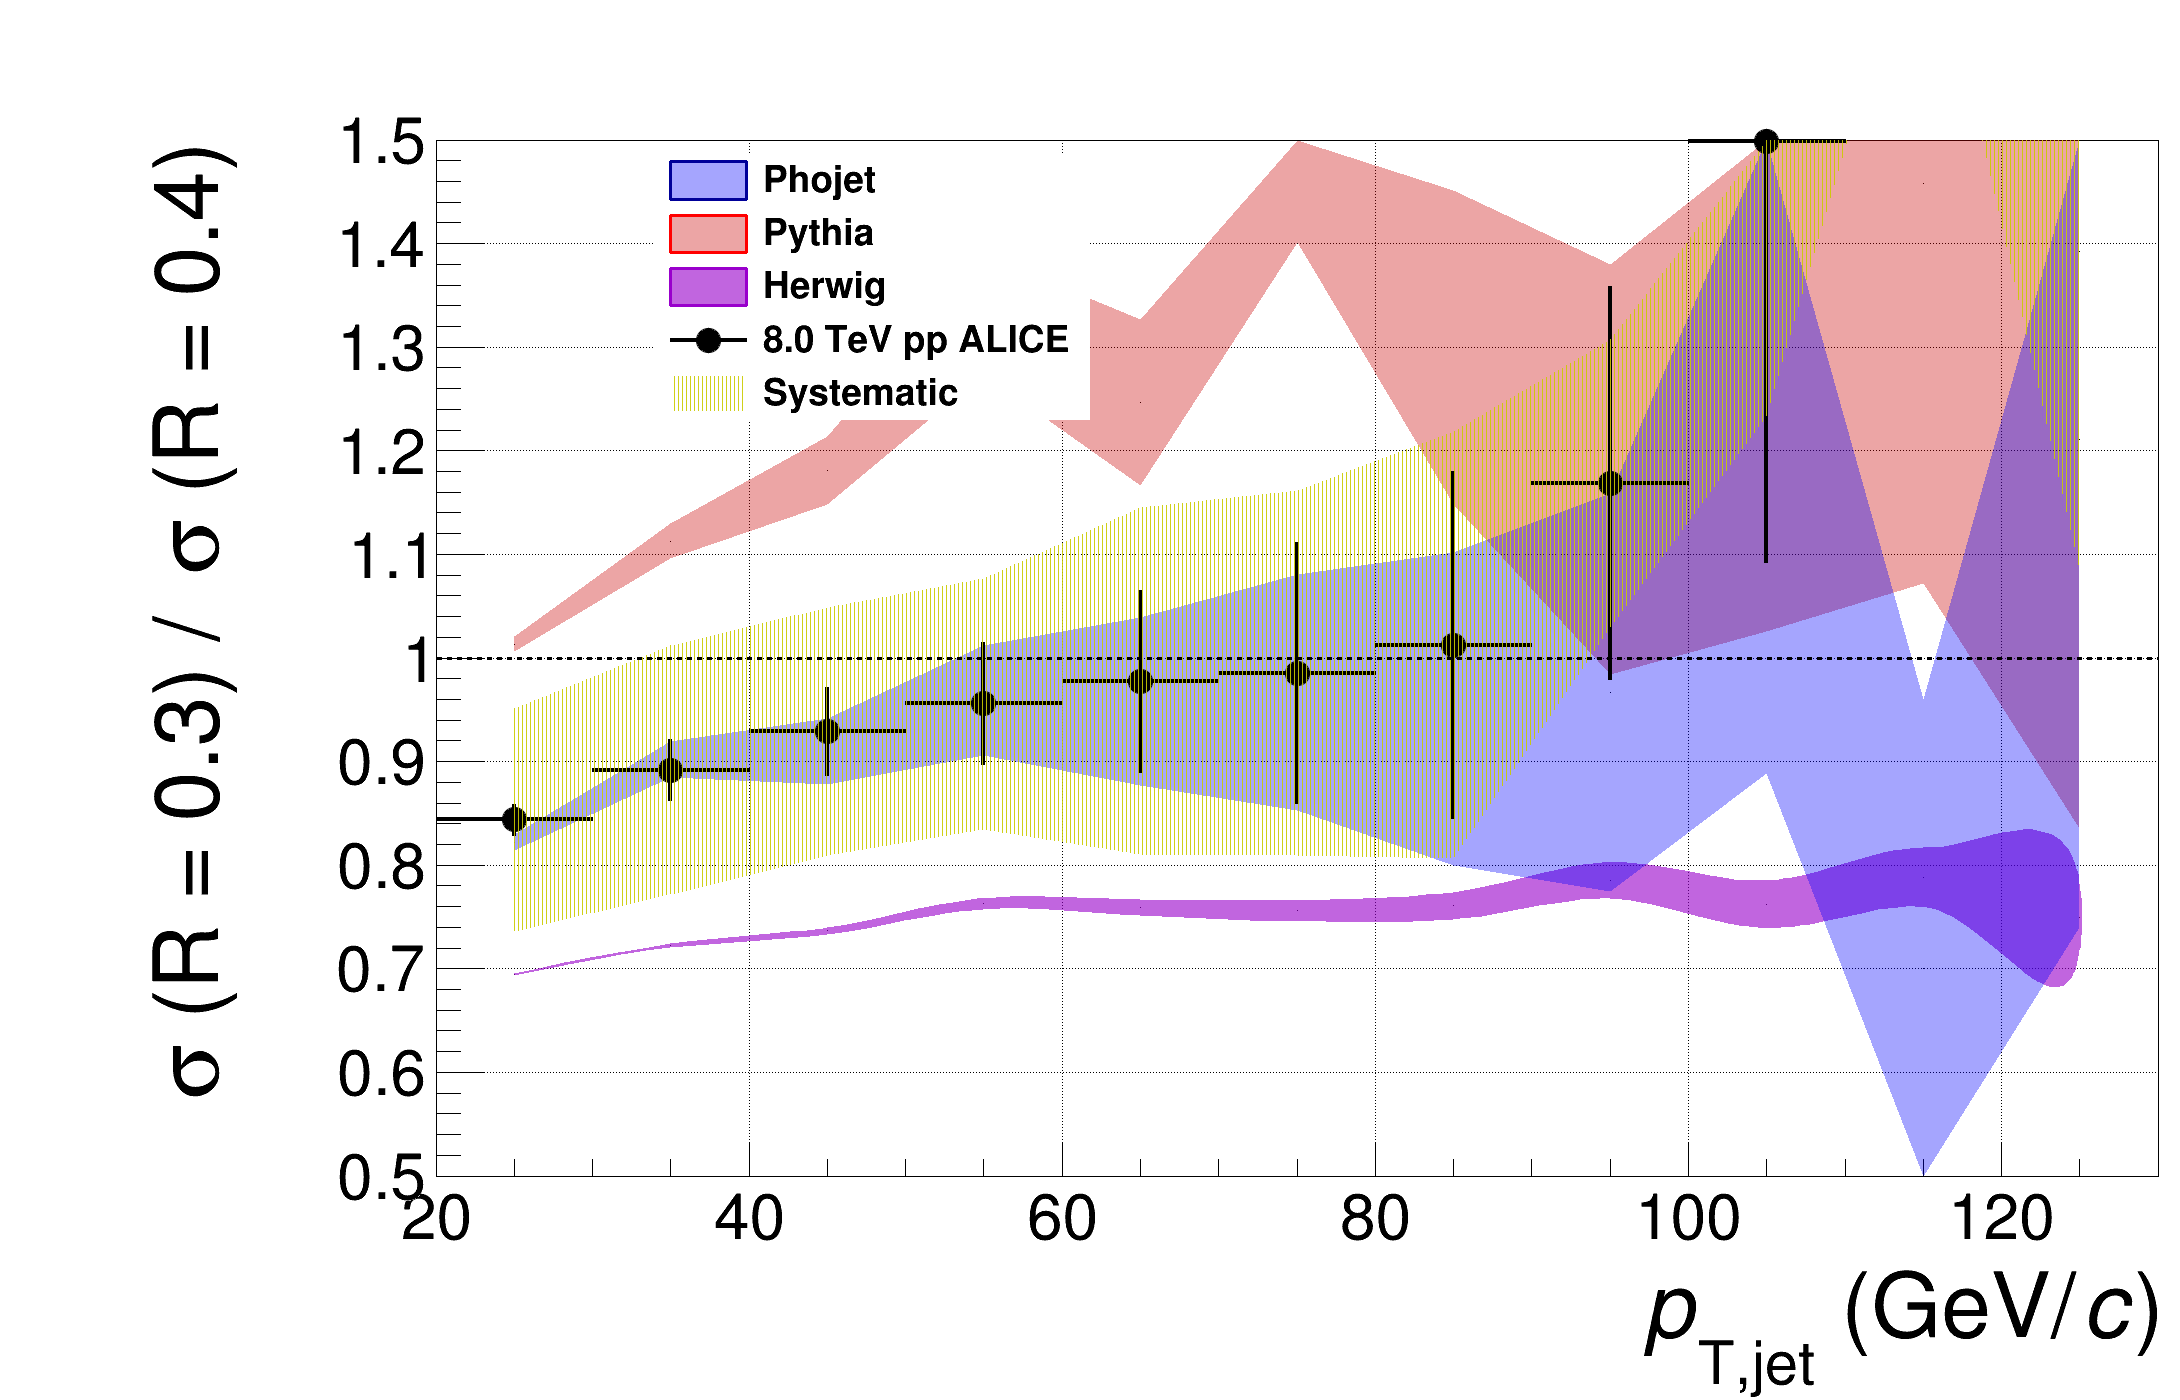
\includegraphics[width=\linewidth]{XSecRatioR03}
\centering
\caption{Ratio of the jet cross-sections R = 0.3  to R = 0.4.}
\label{fig:JetXsecRatioR03}
\end{figure}


\begin{figure}
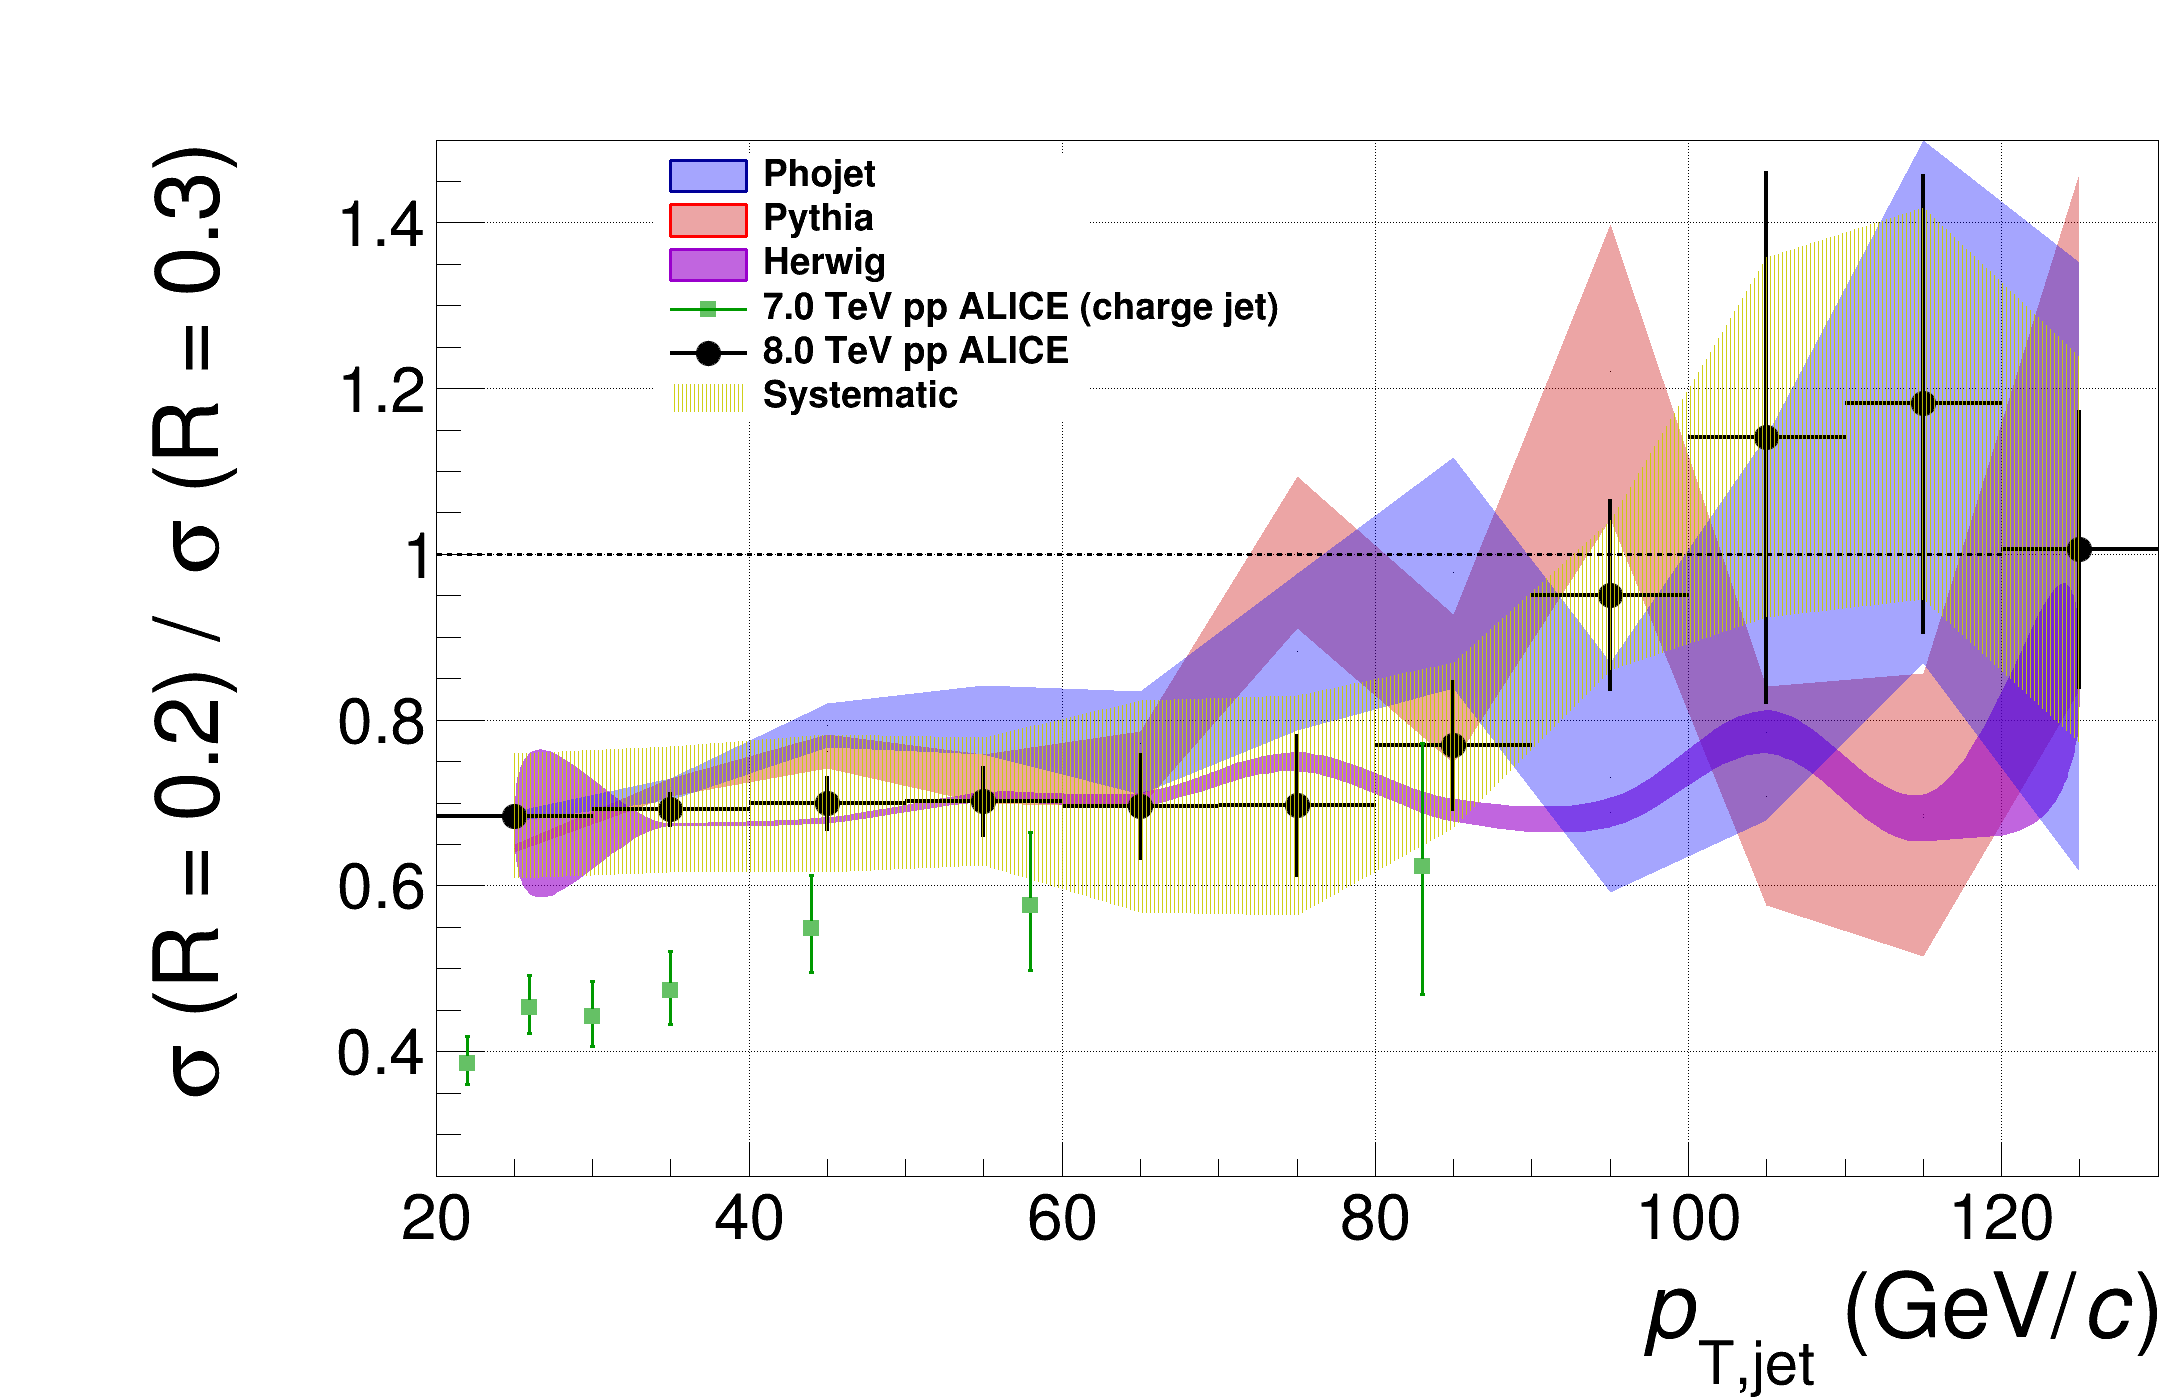
\includegraphics[width=\linewidth]{XSecRatioR023}
\centering
\caption{Ratio of the jet cross-sections R = 0.2  to R = 0.3.}
\label{fig:JetXsecRatioR023}
\end{figure}

\clearpage
}


A similar analysis to this thesis was performed using a 2.76 TeV  data sample collected from ALICE\cite{MA2013319} and it is compared to Figure \ref{fig:JetXsecRatioR02} and \ref{fig:JetXsecRatioR023} in green bullet points.  In order to avoid double counting by sampling the same jet  found using an R = 0.2 and R = 0.4 jet finder these ratios use disjointed samples of the 8 TeV data set.  From the results of the cross-section ratios, we see that the 8 TeV data as reported from this thesis agrees well with the 2.76 TeV results in Figure \ref{fig:JetXsecRatioR02}.  Interestingly it seems that the PHOjet Monte Carlo agrees well with the data for all three figures and is the simulation that agrees the best for the $\sigma (R = 0.3)$ / $\sigma (R = 0.4)$ ratio.  It can be concluded that the Pythia ratios have the least agreement because it only includes the LO matrix to calculate partonic showers, which does not model the angular ordering of QCD radiation very well.  Herwig tends to under predict the data, especially at low-$p_{T}$, which is expected and may be understood in terms of limitations modeling low energy background particles with tune used in this thesis (v2.3).  

Similar to the previous results these ratios can be used to constrain jet quenching in the QGP.  These results also report the first ratio of jet cross-sections between R = 0.2 and R = 0.3.  This is especially helpful for heavy-ion collisions as most jet results from heavy-ions use either an R = 0.2 or R = 0.3 jet radius to suppress the background in the high multiplicity environment.


\section{Conclusion}

Jet cross-sections are a result of QCD interactions while the ratios of the cross-sections for jets of different radii probe the hadronization process.  The essential nature of how hadronization effects the jet cross-sections is still an open question and should be probed in future measurements at the LHC.  ALICE is in the unique position of being able to reconstruct full jets over a wide kinematic range, especially to low momentum.

This thesis presents the first measurements of inclusive full jets at $\sqrt{s} = \,$ 8 TeV using the ALICE detector.  It also presents a procedure, by which using a set of corrections and QA criteria, we may obtain results comparable to pQCD Monte Carlo simulations.  The agreement between the results and Monte Carlo simulations show the jets are a well calibrated probe for testing QCD phenomena.  In terms of the kinematic reach, the results of this thesis are in good agreement with QCD calculations down to 20 GeV/\textit{c} through 100 GeV/\textit{c} in $p_{T}$.  This range may be extended with better Monte Carlos in the furture and this is currently being worked on until the results are published.  With a better Monte Carlo production we could see the range extend to between 5 GeV/\textit{c} to about 200 GeV/\textit{c} in $p_{T}$.  The comparisons with the Monte Carlos agree well, with the most tension lying with PHOJET.  However, these results are expected to improve once an improved GEANT4 Monte Carlo that models the EMCal trigger is made available.  

It is striking how well both hadronization models, the Lund-String model and Clusterization model encompassed by Pythia and Herwig, agree with the data.  These are fundamentally different physics phenomenology and it begs the question , why this is?   It is interesting and exciting that some of the initial questions posed when I started my Ph.D. work remain and I am hopefully for new insights from future work in both theory and experiment.  

The results from this thesis can also be used in future heavy-ion runs to probe jet quenching, as these results would serve as a baseline comparison.  The work in this thesis also presents the jet measurements from ALICE down to 20 GeV/\textit{c}, which will be important for probing energy loss in the QGP.  By measuring these very low energy jets we can probe the full energy loss mechanism for partons traversing the QGP.  Previous higher energy jet results would tend to bias to jets that traveled a very short distance through the QGP.

With the increase in energy and luminosity seen at the LHC, we have moved into the era of high-precision testing of pQCD.  The work set forward by this thesis sets the stage for using jets in the future at CERN, especially after the high luminosity upgrade of the LHC is complete.  Although it dates to 2012, the 8 TeV contains some of the largest data sets available at a given energy from the LHC.  This makes it an important data set and worthy of future investigations.  I'm proud of the work presented in this body, both in terms of the data analysis and engineering aspect.  What results we will gain from the upgraded LHC and jets is only left to our imagination and to nature's mercy.